\subsection{VALOR POTENCIAL CON EXPLOTACI\'ON DE OPORTUNIDADES EXTERNAS.}
 
Se llev\'o a cabo la valuaci\'on de \textcolor{principal}\descripcionBien} a partir de la informaci\'on de negocio y financiera proporcionada por el solicitante, habiendo aplicado el marco te\'orico de la valuaci\'on de negocios; bajo el punto 4 del pent\'agono de explotci\'on de oportunidades conocido como \textit{``Valor potencial con mejoras externas´´}  (\textcolor{terciario}{\autoref{fig:hexagono}}).

\begin{figure}[H]
\centering
\caption{Pent\'agono de Explotaci\'on de oportunidades\label{fig:hexagono}}\vspace{10pt}
\includegraphics[width=7cm]{\rutaImagenes/pentagono}\\
Fuente:Valuation. Copeland Tom, Koller Tim y Murrin Jack.\\

John Wiley \& Sons. 1995.
\end{figure}

``\textcolor{secundario}{Valor potencial con explotaci\'on de oportunidades externas}.- Es el valor que adquiere la unidad econ\'omica valuada una vez que se realiz\'o la identificaci\'on y explotaci\'on de los factores externos. Para lo cual se corrigen deficiencias, se mejoran y optimizan procesos y se explotan nuevas oportunidades estrat\'egicas, obteni\'endose as\'i un mayor valor de la unidad econ\'omica''\\

